% This example An LaTeX document showing how to use the l3proj class to
% write your report. Use pdflatex and bibtex to process the file, creating 
% a PDF file as output (there is no need to use dvips when using pdflatex).

% Modified 
\documentclass{l3proj}

\usepackage{subcaption}

\begin{document}

\title{Leidos Roll Vans Project}

\author{Filip Vyrostko \\
        Alen Reji \\
        Ewan Bell \\
        Harsh Kheskani Raisinghani}

\date{March 2022}

\maketitle

\begin{abstract}

In this paper, we present a case study of the software development process of the Roll Vans web application created for Leidos company as part of Team Project 3 coursework.


We describe the process itself as well as practices used during its development.


The paper describes our most prominent learning achievements as well as the evolution of our understanding of key areas of the development process, such as Issue Management, Code Reviews, Version Control, Customer Communication, etc.

 
Moreover, we compare existing software engineering practices with those employed by us during the process and reflect on the advantages and/or disadvantages of these practices.

\end{abstract}

%% Comment out this line if you do not wish to give consent for your
%% work to be distributed in electronic format.
\educationalconsent

\newpage

%==============================================================================
\section{Introduction}

Software engineering 

This paper presents a case study of Agile practices and how they were employed for our Roll Vans web application. It is a record of how successful we were in implementing these practices to provide a complete and satisfactory application for Leidos. The paper also includes our reflection on how each practice was incorporated and how each practise impacted our development team and the product itself.


%% Final paragraph.
The rest of the case study is structured as follows.  Section
\ref{sec:background} presents the background of the case study
discussed, describing the customer and project context, aims
objectives and agreements and the project state at the time of writing.
Section \ref{sec:customer} involves our interaction with the client throughout the software process.
Section \ref{sec:dev_process} discusses areas of the development process employed by our team in which we found value as well as documenting the encountered challenging areas and our resulting improvements. Lastly, section \ref{sec:deployment} describes deployment, the final step of our development life-cycle. 

%==============================================================================
\section{Case Study Background}
\label{sec:background}
    This section provides background for Leidos, its initial product proposal (section \ref{sec:proposal}), our changes to that proposal, as well as our implementation choices (section \ref{sec:imp_and_agr}). Lastly, in section \ref{sec:delivered}, we discuss our delivered product and its intended use by the customer.
    
    %------------------------------------------------------------------------------
    \subsection{Client and Proposal}
    \label{sec:proposal}
        Leidos is a large, multinational organization looking for a way to bring small, independent businesses into the marketing spotlight without the use of conventional marketing platforms, all without a fee.
        

        The main idea behind this project was to introduce a platform for small, independent businesses, in order for them to create an online presence. The reason for this being that popular marketing platforms such as Google are simply not an option due to the price for the marketing as well as there being a large amount of competition.

        

        The initial proposal suggested an Android and/or iOS mobile application, with integrated maps API to overlay locations of businesses on a map. On top of that, it was required for each business to be able to create their own profile with appropriate information such as name, address, description, menu and opening times. Moreover, the application should support push notifications for subscribed locations, allow notifications to snooze for varying time periods, be lightweight in its performance and requirements and use modern UI design.
        Lastly, the proposal hinted on possible inclusion of a rating/review system as well as integrated social media sharing and UI space dedicated to advertising for revenue purposes.
        %------------------------------------------------------------------------------
    \subsection{Implementation Goals and Agreement}
    \label{sec:imp_and_agr}
        After the first customer meeting, it was agreed that despite the initial proposal of an Android/iOS mobile application, our team will develop a web application instead. This decision was taken due to our concerns of no prior knowledge of mobile application development.
        

        Due to the change in platforms, our team decided to create a new list of requirements based around a web app rather than a mobile app. We decided to drop mobile application specific features such as 'support for push notifications for subscribed locations' or 'allow notifications snooze for varying time periods'. Nonetheless, we were able to retain most of the features from the original proposal. After getting a green light from the customer on the new list of features, we have presented them with the framework intended for the development as well as arguments for the choice. We decided to use the \textit{Django} (web application framework) \cite{django} framework with its primary language being \textit{Python}.

        

        Looking at the choice of framework now, it shows our inexperience in field of web development, as using \textit{Rest Framework} \cite{rest} for Django with \textit{Angular} \cite{angular} or \textit{React} \cite{react} as front-end frameworks would have been a much better choice as this was a more standard approach in the industry and would have also given our project more usability and customizability.
        
    %------------------------------------------------------------------------------
    \subsection{Delivered Application}
    \label{sec:delivered}
        Our delivered web application will not be mass deployed publicly. The main purpose was to create a prototype for the customer to use as a stepping stone in further development, as well as to see if this idea had any potential (will be presented to some real users). The prototype would be hosted online and the link shared between the team and the customer only, as per the customers requirements. This was to ensure constant feedback from the customer as well as the customer being able to see the prototype progressing. 


%==============================================================================
\section{Customer Interaction}
\label{sec:customer}
    This section outlines our interaction with Leidos. It describes how we used the customer meetings to form requirements (section \ref{sec:req_and_feat}), how we structured our customer meetings (section \ref{sec:communication}) and what we took away from each meeting (section \ref{sec:retrospectives}).
    
        %------------------------------------------------------------------------------
    \subsection{Forming Requirements and Features}
    \label{sec:req_and_feat}
        As already mentioned in section \ref{sec:imp_and_agr}, we had to create our own list of features and their priorities on top of the list proposed by the customer. Both original and modified requirements lists were very specific. To better outline the functionality, we have decided to use user stories. As per the proposal, two main user figures arose, a customer and a business owner. Each story focus on one of the two figures, describing their needs and wishes. By constructing these stories, we were able to effectively establish required functionalities and reasoning behind them.
        

        

        After forming the list of features, we decided to create a priority list in order to identify what we believed should be focused on first. For this, we decided to use MoSCoW \cite{moscow} method as prioritization technique. This prioritization was later presented to the customer and after their agreement, we proceeded to use planning poker (\textit{planITpoker} \cite{poker}) to estimate time to develop for each feature. Planning poker is a team exercise wherein team members estimate the amount of time taken for each feature to be implemented, before comparing their times with the rest of the team, allowing members to justify and explain their thought process before the team collectively agree on a set time.
        

        

        We concluded that our user stories proved to be very beneficial in defining features from the end-user point of view and solidifying our reasoning behind each feature. Similarly, the MoSCoW principle also proved to be crucial in defining priorities for each feature and together with other implemented techniques, helped us effectively create an efficient timetable for our development. Despite this, our inexperience showed, and we missed several important user stories which in effect broke the timing estimates for development of some features. For example, we considered a user story for a user viewing a business page however, we had completely neglected how the user gets access to the business page (i.e. navigation bar). If we were to redo this now, we would more closely follow steps suggested by Lawrence and Green \cite{stories}, and split the story more thoroughly, likely uncovering smaller features that need to be implemented rather than large sized and very general chunks as well as create user stories describing changes across all architectural layers, not just one. Looking back, we also now realise that generating a sitemap \cite{map} ahead of development would have allowed to further think about navigation and divide the website structure better and analyse the smaller components which were not covered explicitly under our broad definitions.
    
    %------------------------------------------------------------------------------
    \subsection{Customer Communication and Meetings}
    \label{sec:communication}
        Early on in our project we had been advised to consider client-team communication; a crucial part of our development process. In order to address this part of the process and trying to follow the Agile principle of \textit{delivering working
        software frequently} \cite{manifesto}, we split our project into 6 iterations. Each iteration lasting roughly a month, at the end of which we presented the customer with our progress.

        Later in the development process, we managed to implement our CI/CD pipeline which further enhanced the already mentioned Agile principles. Furthermore, it gave us the opportunity to employ another Agile principle, namely the principle of \textit{changing requirements} \cite{manifesto}, as we were able to receive constant feedback from the customer as the application had been deployed using the pipeline, allowing the customer to see the changes effective immediately. This sometimes changed the requirements for the sprint while it was in progress, as the customer would provide valuable feedback which we were able to use to alter the website and make it more satisfactory.

        

        Each iteration (sprint) meeting focused on the presentation of the progress since the last meeting and the current state of the project. This was followed by feedback from the customer and then a discussion on the set of deliverables for the next sprint.
        
        \begin{center}
            \begin{table}[H]
                \centering
                \begin{tabular}{ll}
                \textbf{Date}      & \textbf{Meeting Purpose}
                \\
                October 13th 2021  & Initial Project Meeting \\
                November 10th 2021 & Iteration 1 Summary     \\
                December 1st 2021  & Iteration 2 Summary     \\
                January 19th 2022  & Iteration 3 Summary     \\
                February 16th 2022 & Iteration 4 Summary     \\
                March 23rd 2022    & Final Customer Day   
                \end{tabular}
                \quad
                \caption{Client meetings}
            \end{table}
        \end{center}
        \begin{center}
            \begin{table}[H]
                \centering
                \begin{tabular}{ll}
                    \textbf{Time}   & \textbf{Purpose}                                 \\
                    5  min  & Introduction to Meeting Content         \\
                    10 min & Demonstration of Our Progress           \\
                    7  min  & Customer Feedback                       \\
                    3  min  & Present Deliverables for Next Iteration \\
                    5  min  & Summarize the Meeting                  
                    \end{tabular}
                \label{tab:my_label}
                \caption{Meeting Timeboxing}
            \end{table}
        \end{center}
        
        

        

        More specifically, our first meeting was used to communicate and present the customer with our changed proposal for the meeting [\ref{sec:req_and_feat}] as well as discuss technologies to be used and licensing choices. Our second customer meeting was used to communicate our conceptual visualization of the proposal via a \textit{Figma} Wireframe. As discussed in article by Fred Wilson \cite{wireframe}, wireframes enhance the adaptability, deepen the collaboration with customers and provide an easy way to facilitate feedback.
        

        

        Our other two communication channels were Microsoft Teams and emails in case direct communication in between iterations (sprints) was needed.
        
        

        

        Despite good results with client-team communication, we had neglected good communication internally, causing one of the features to be delayed into the next sprint. Although we covered the deliverables for the next sprint with the customer and notes were taken on this, not all of these had been created as issues on GitLab, our DevOps platform, causing us to forget about some features when planning our time allocations. There were also some issues with merging branches and pushing/pulling code as we sometimes did not flag that new code was pushed, causing merge errors and code alteration when another team member tried to push code later on. After this, communication was flagged as top priority, and we decided to hold at least one Teams meeting a week and an in-person mob/pair programming session every Wednesday (more on these sessions in \ref{sec:mob}). This greatly improved communication between our team and the in-person meetings greatly improved team cohesion and reduced confusion because if one team member ran into an error, especially with someone else's code, the rest of the team were there on-site for aid.
        
        

        

        Overall, these practices greatly helped us to reduce any miscommunication from happening. However, we have to admit  our customers were good at communicating their requirements and so maybe this was not that reflective of the 'real world'. Nonetheless, there were few incidents where direct communication with customer was very slow. For example, when deciding on colouring of the page, email was sent to customers asking for their input. The response came fairly late, however we were able to adapt to it quickly. As for meetings themselves, we had implemented strict time boxing in the later part of the development as a result of one of our retrospectives[\ref{sec:retrospectives}]. This increased the value of the sprint meetings even further, as they were more on point, thus reducing miscommunication or discussions on topics of a lesser priority.

        In retrospect, if we were to make some changes to our communication and planning, we would probably split the last two iterations into 4 as suggested by extreme programming methods \cite{ep} and would seek to establish more frequent and stable communication loops. This decision is in regard to increased work load and the number of features implemented in last two sprints, thus increasing the need for more frequent feedback from the customer.
        
        
    %------------------------------------------------------------------------------
    \subsection{Post Meeting Reflection}
    \label{sec:retrospectives}
        Within two days after each meeting, a retrospective was held, as to promote the Agile principle of \textit{the team reflects on how to become more effective at regular intervals} \cite{manifesto}.

        Initially, we just discussed and repeated the customers feedback from the meeting but, after learning that we needed to be more in-depth, we decided that after each retrospective, we would go over the iteration and classify all that happened as either \textit{Went Well} or \textit{Went Wrong}. Next we would focus on things that went wrong and used the \textit{5 Why's} \cite{whys} method to understand the root cause of the problem. After we understood what went wrong in more detail, we would discuss how to improve it. Improvements would be then classified as \textit{How to Improve}.
        

        

        Overall, our team agreed that this was probably the most valuable thing we learned in the entire development process as it was the root cause for learning and employing other practices. For example as later discussed in section \ref{sec:mob}, we decided to improve our team communication by actually meeting in person for some mob/pair programming. This not only strengthen our team bonds but also greatly improved communication and promoted the Agile principle of \textit{most efficient and effective method of conveying information to and within a development team is face-to-face conversation} \cite{manifesto}.

        Nonetheless, it took us a while to understand how to properly hold retrospectives. For example as discussed in article by Sean Blake \cite{retro}, you should \textit{review your action items at the next retrospective}. We did not do that initially and merely created new action items for each. Our coach however, had brought up this problem and discussed the quality of retrospectives and how it could benefit the development process. After that we employed the more thorough approach as stated above. This then reflected on the quality of retrospectives and we were able to identify some recurring problems and the actions needed to be taken to sort these problems. 



%==============================================================================
\newpage
\section{Development Process}
\label{sec:dev_process}
    In this section we give insight into our development process. 
    From section \ref{sec:version_control} to section \ref{sec:cicd} we describe our development practices such as Issue Management, Mob and Pair Programming, Code Reviews and CI/CD Pipelines.
        
    %------------------------------------------------------------------------------
    \subsection{Issue Management}
    \label{sec:version_control}
        Version control was used to manage workflow of our project. Each feature was translated to an issue, where each issue was worked on by 1 or more team members. In addition, for each issue, a branch was created which was then merged with master once it was fully developed.

        Issues were assigned to each team member based on preferences as well as experience and estimated time to complete to balance the workload. In order to better estimate time, we have use planning poker using \textit{planITpoker} \cite{poker} web application. This helped us to better understand how to balance the workload, which simpler task can be put together and which more complex task could be split apart.

        Once a feature branch was complete, in order to be passed to master branch, it had to pass CI/CD pipeline (more in section \ref{sec:cicd}). After that, exhaustive merge message was written in order to help code review. We tried to follow the guide by Caleb Hearth on how to write appropriate commit messages and apply it to merge requests too \cite{commit}. This was not what had been happening initially as at first, we had poor commit messages which were usually only one line. This caused issues as the message did not fully explain the changes that had been made to other team members who later were trying to work on the same branch. After improving our messages, using the guide mentioned above, our development flow became smoother as other teammates did not need to contact the commit author repeatedly to double check what exactly had been altered. Also, the new commit messages included changed files which were great in reducing merge conflicts when pulling code as one could check the commit messages beforehand to see which file would be changed when pulling and could then stash or discard the local changes accordingly.

        \begin{figure}[H]
            \begin{subfigure}{0.5\textwidth}
                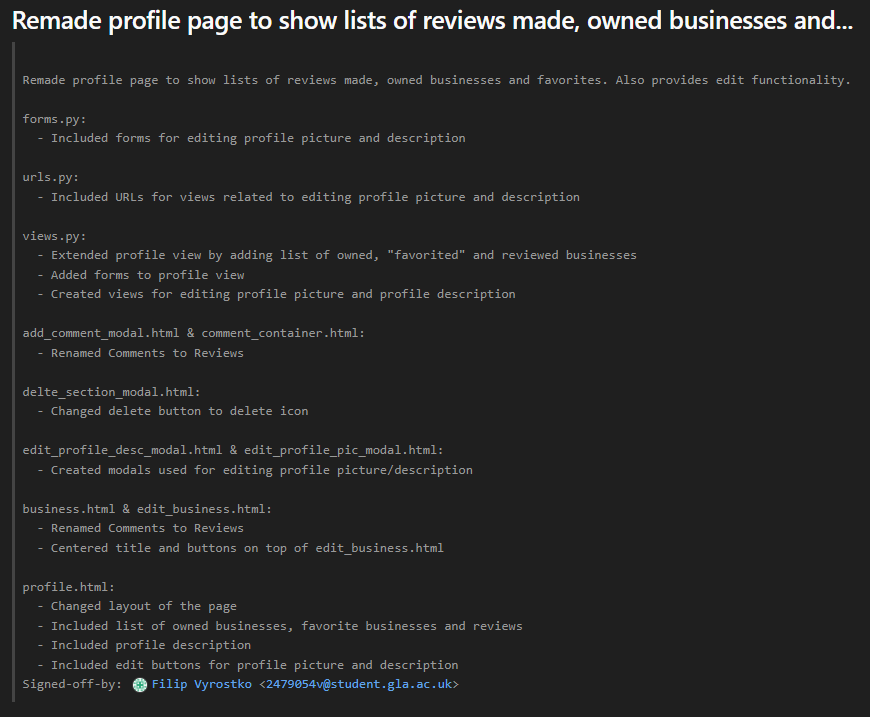
\includegraphics[width=0.9\linewidth, height=6cm]{images/CommitSnippet.PNG}
                \caption{Commit Message}
                \label{fig:commit_msg}
            \end{subfigure}
            \begin{subfigure}{0.5\textwidth}
                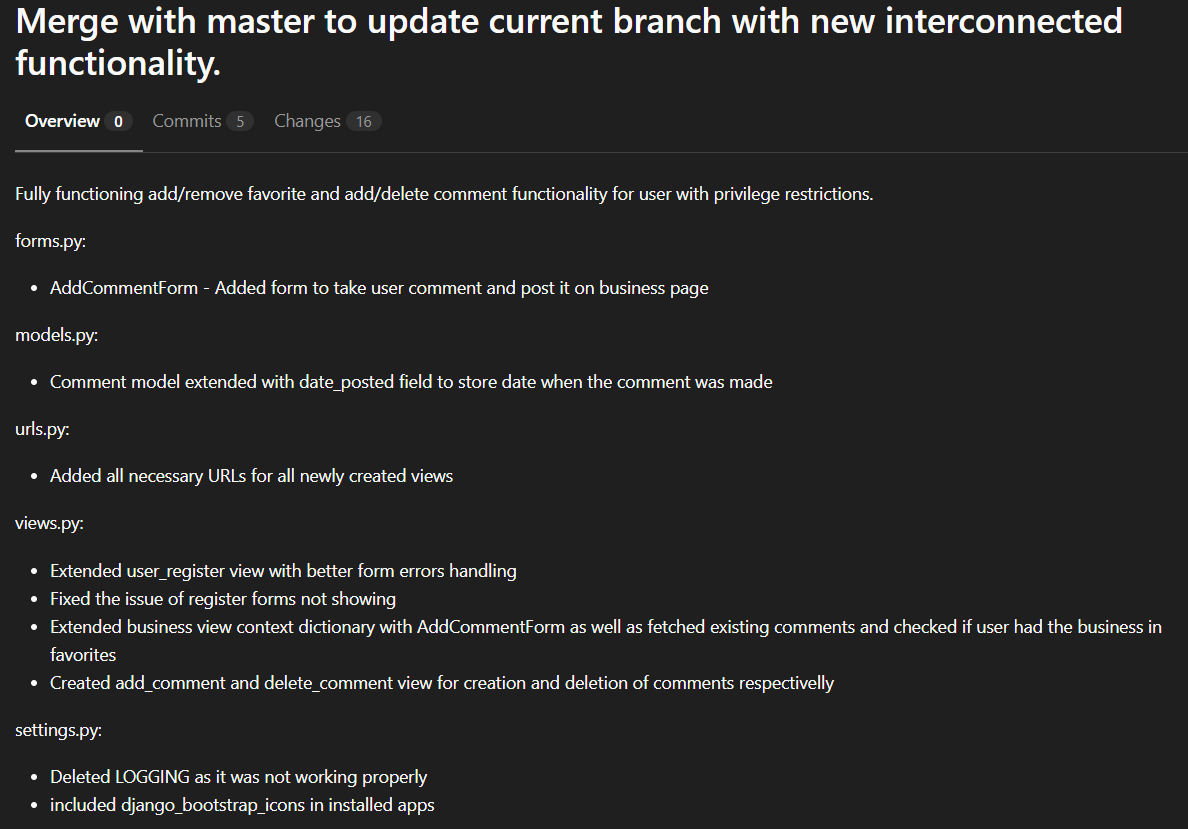
\includegraphics[width=0.9\linewidth, height=6cm]{images/MergerSnippet.PNG}
                \caption{Merge Message}
                \label{fig:merge_msg}
            \end{subfigure}
            
            \caption{Structural example of commit and merge messages used throughout the project}
            \label{fig:image2}
        \end{figure}
        Overall, the practices we employed helped us reduce merge conflicts and make it clearer what had been done for the person conducting the code review. Nonetheless, we still faced some conflicts at the end which slowed down the merging process. Moreover, we initially did not do proper code reviews (section \ref{sec:mob}) and mob programming sessions. This was corrected later on in the development process. Additionally, we have employed \textit{Merge down/Copy up} Agile approach for merging as described in article by Steve Berczuk et. al. \cite{merge}.

        In addition, we recognize the lack of continuous time management via planning poker as suggested in article by Mike Cohn \cite{continuous_poker}. In hindsight, some of our estimates were too optimistic and reflect our inexperience. Moreover, as already mentioned in section \ref{sec:req_and_feat}, our user stories were incomplete and lacking in some areas. Hence, we believe if we were to hold planning poker more frequently (together with complete user stories), we could have avoided some workload inequalities.
        
        
        
    %------------------------------------------------------------------------------
    \subsection{Mob/Pair Programming and Code Reviews}
    \label{sec:mob}
        Our team practised weekly mob/pair programming sessions after one of the retrospectives (section \ref{sec:retrospectives}) as well as to promote the Agile principle of \textit{most efficient and effective method of conveying information to and within a development team is face-to-face conversation} \cite{manifesto}. Initially, we held only mob programming sessions as pair programming requires one or both programmers to be proficient in their area. Through the mob programming we were able to teach one another different parts of the framework, thus creating a deeper understanding of the interconnected workings of the framework. This in turn helped team members predict how some parts of the project might change with respect to changes in others.

        Once we were confident in the abilities of each team member, we started with pair programming sessions.

        Lastly, each session ended with group code review. In case of pair programming, one of the drivers for the pair would go over the code written and explain its workings. This made it less likely code which had logical error and flaws would be pushed without corrections. Moreover, this enforced another Agile principle of \textit{working software is the primary measure of progress} \cite{manifesto}. Again, this process was not what we had done initially as we did no code reviews at the start. After receiving some feedback from our coach and understanding code reviews and their benefits, we decide to do them weekly after each in-person session. These code reviews were very beneficial as they broadened our understanding of the framework used. However, as mentioned in article by Dan Radigan \cite{code_review}, we could have used code reviews to better estimate how long each task takes, thus catching the issue mentioned at the end of the section \ref{sec:version_control} early. Unfortunately, we did not do that, which cause an inadequate work load. Now, we believe that we would be able 
        to better facilitate these reviews and sessions and possibly correct some of the mistakes made in different parts of development.

        
        Overall, our team enjoyed both mob and pair programming sessions. Unfortunately, we were unable have such sessions in the first semester due to COVID-19 and other problems which cause a team member to be unable to be in Glasgow. Nonetheless, in the second semester we were able to use these to our advantage. 
    %------------------------------------------------------------------------------
    \subsection{CI/CD Pipeline}
    \label{sec:cicd}
        The main goal for our CI pipeline was to ensure that the project was in working state through concurrent development. In addition, it further enforced the Agile principle of \textit{working software is the primary measure of progress} \cite{manifesto}.

        Each branch when merged into the master, had to pass the CI pipeline. In the case that the pipeline failed, the issue was investigated and fixed as soon as possible.

        As for CD pipeline, we initially used one in separate deployment branch for deployment of our web application on \textit{Heroku} \cite{heroku}. Initially, we found great benefit in using this as once we had merged a working feature into master we could just clone this into the deploy branch and it would automatically push the changes to Heroku. Nonetheless, as mentioned later in the paper (section \ref{sec:deployment}), we had to remove it.

        
        Overall, our experience with CI/CD pipelines are mixed. This could be attributed to the fact we had a hard time to setting it up and getting it to properly work or that the automated deployment platform we selected (\textit{Heroku}), did not fulfil our needs. The CI/CD pipeline itself did not impact too much on our small project, other than automating the running of tests as automated deployment was not possible further down the line as we decided to not use Heroku for deployment, and we had wasted some time in learning to use the GitLab CI/CD with Heroku. However, if this project were much larger, the pipeline would be crucial in saving time with testing and deployment. Moreover, we found the already mentioned approach of 'Merge down/Close up' \cite{merge} to be more effective in ensuring working branches and effective merging into master. Nonetheless, we see the value in CI/CD pipelines, namely in CD for automation of deployment phase. Each of our team member will certainly consider using pipelines in the future projects.
        
    %------------------------------------------------------------------------------


% ==============================================================================
\section{Deployment Process}
\label{sec:deployment}
    We had initially deployed our application using \textit{Heroku} \cite{heroku}. This proved to be problematic as our web application heavily relies on visual elements such as images which were not present on Heroku. However, for the period of time we had our application deployed there, we utilized the CD pipeline for immediate deployment of recent changes which in turn allowed rapid feedback from the customer throughout development.

    Later, we had decided to deploy our application on \textit{PythonAnywhere}\cite{pythonanywhere}. Unfortunately for us, PythonAnywhere does not support CD pipelines. Thus, whenever there was a change we had to manually pull from our repository to PythonAnywhere. After having a team discussion about the trade-off between Heroku and PythonAnywhere, we unanimously agreed that having media on our site would be crucial in our ability to deliver a well-rounded and satisfactory application to the customer and that this was more important than being able to save some time with automatic deployment.
    
    Our handover process was straight forward. We had agreed with the customer to provide them with full access to our repository, as well as host the application and give them access to the hosting account as well. Moreover, our customer requested we provide a documentation on how to work with the web application as well as what are some know bugs and quirks and how to avoid them. This document was created and emailed to them.

    In terms of licensing, our customer delegated the entire responsibility to us. Therefore, in light of the expected usage of our application mentioned in section \ref{sec:delivered}, we have decided to use \textit{Permissive} \cite{permissive} licensing, namely \textit{Apache license 2.0} \cite{apache}.
    

%==============================================================================
\section{Conclusion}

In this dissertation, we covered our first taste of a professional software development process and how we handled interaction with a real-world customer. We outlined the methodologies we used both in the planning stage and the development stage and how these methodologies affected our process and also discussed why they worked or didn't work. The challenges that we encountered along the way are also highlighted as well as the actions we took to correct them and the reasoning behind those actions.

Throughout the process, our inexperience as developers as well as our unfamiliarity with the process was apparent. Although this did cause some issues throughout, we sought to rapidly correct this after receiving feedback or experiencing some failure. We learned that development is not just writing code, it includes many other sub-processes some of which, although seeming insignificant, makes a huge impact on how well a development team is able to perform. Yet another alien experience was working as a team, especially working with code written by others and writing code with others in mind. Eventually we were able to achieve cohesion and make the development process move smoothly. What we learned most is that the development process involves constant refinement, whether that be in writing code, documentation, communication, etc. We continuously have to be thinking about making things better. 

%==============================================================================
\bibliographystyle{plain}
\bibliography{dissertation}
\end{document}
